\section{hash functions}

\begin{frame}
	%\frametitle{Was sie tun}
	\frametitle{what they do}
	%Eigenschaften
	Properties:
	\begin{columns}
	\column{6cm}
		\begin{itemize}
		%	\item Surjektiv \begin{small}(Eindeutige Abbildung)\end{small}
		%	\item Kollisionsfrei
		%	\item Lawineneffekt
			\item surjective \begin{small}(unidirectional projection)\end{small}
			\item collision free
			\item good averlanche-effect
		\end{itemize}
	\column{6cm}
		\begin{center}
			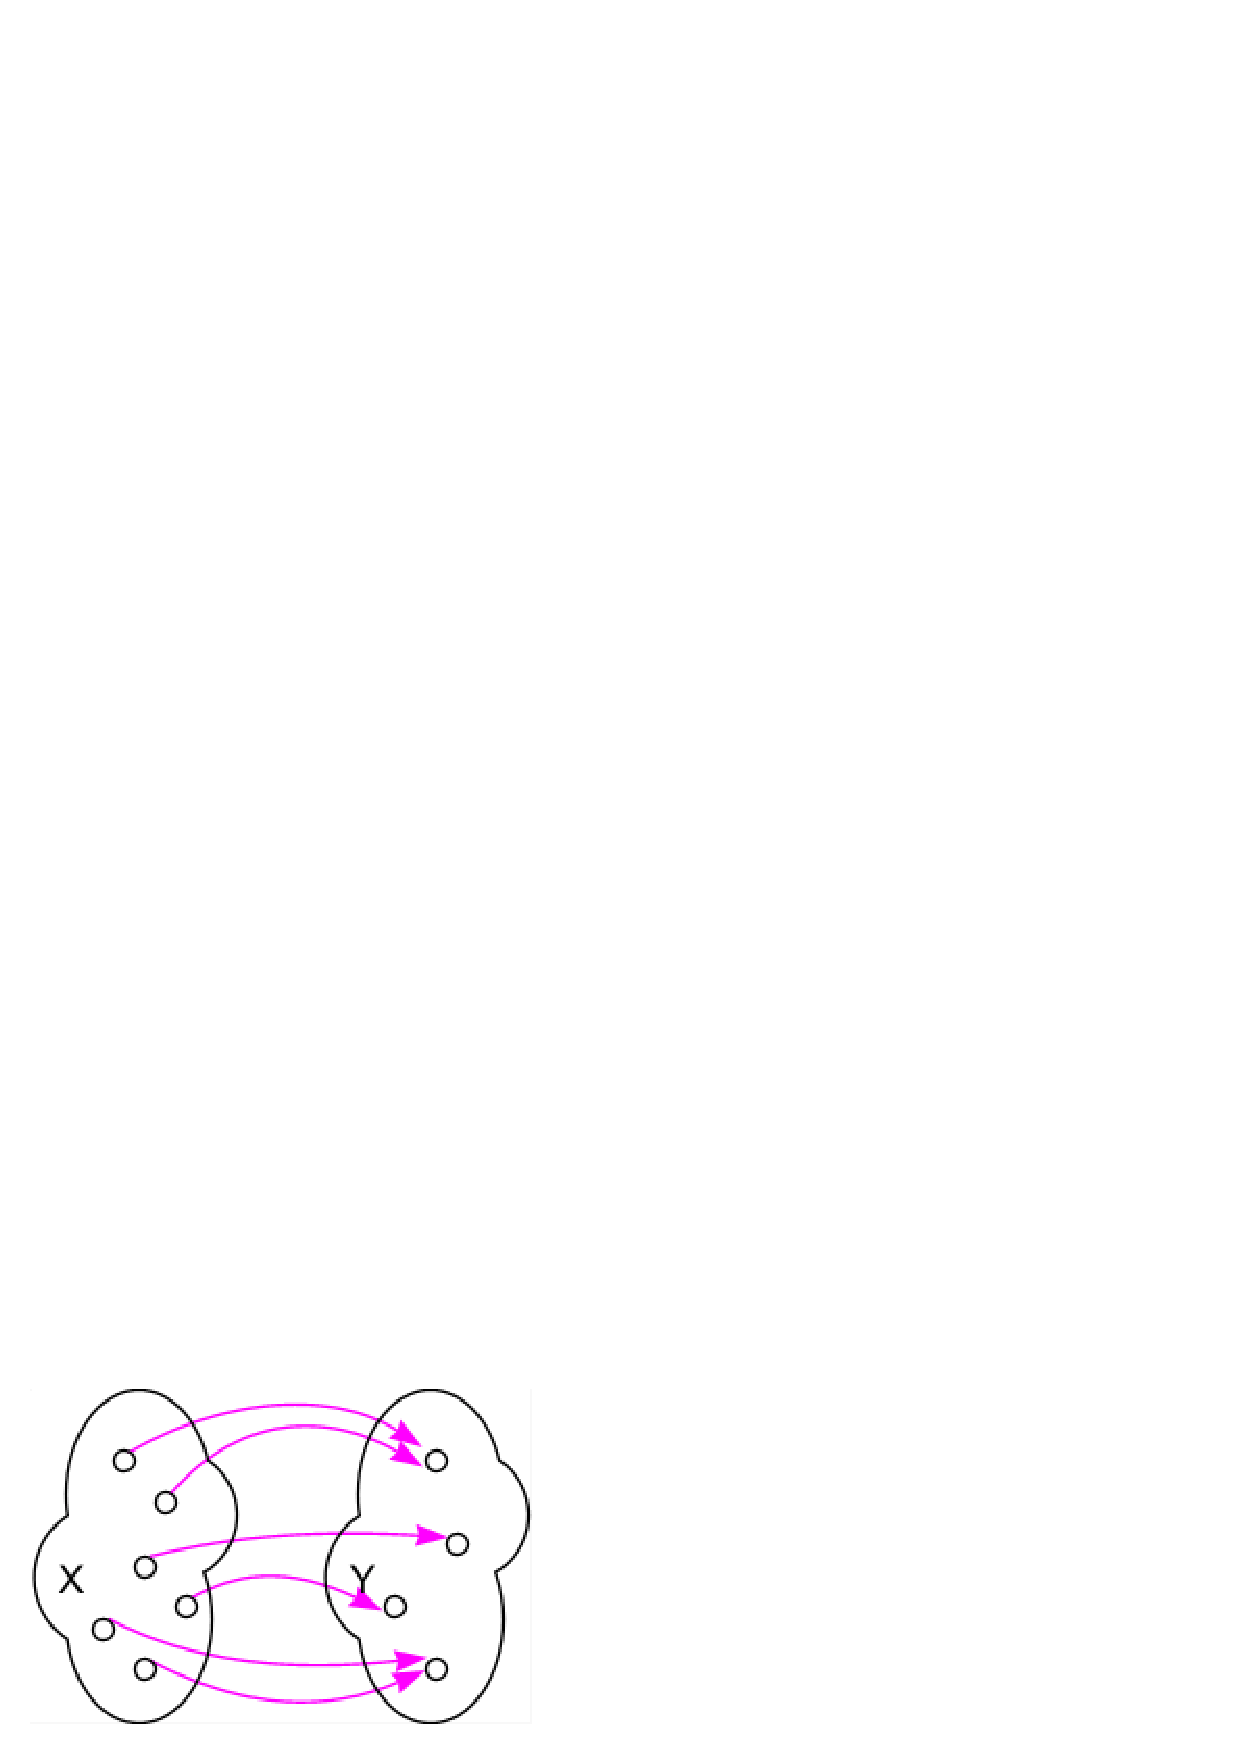
\includegraphics[width=4.8cm,height=3.2cm]{surjektiv}
		\end{center}
	\end{columns}
\end{frame}

\begin{frame}
\frametitle{what for?}
	\begin{columns}
	\column{6cm}
		\begin{itemize}
			\item One-way property
			\item useful for large messages
		\end{itemize}
	\column{6cm}
		\begin{center}
			
\includegraphics[width=4cm,height=6cm]{oneway}
		\end{center}
	\end{columns}
\end{frame}

\begin{frame}
\frametitle{example of usage (1)}
	secure storage of passwords
	\par
	\begin{center}$hash( seed \parallel passwort )$\end{center}
\end{frame}

\begin{frame}
	\frametitle{example of usage (2)}
	Alice and Bob want to make a decision, where there normaly would flip a coin for.
	But they can not meet and have only a halfduplex communication channel (ex. a telephoneline).
	\begin{enumerate}
		\item<2-> Alice generates a random bitstring $m$ of sufficient length (ex. 512 bit) and keeps it secret
		\item<3-> Alice sends Bob the hash value $h(m)$ of $m$
		\item<4-> Bob ''guesses'' the value of the least significant (or other well defined) bit and sends his guess to Alice
		\item<5-> Alice now sends $m$ to Bob
		\item<6-> Bob validates that the recieved hash matches the hash of the recieved bitstring $m$
	\end{enumerate}	
\end{frame}

\begin{frame}
\frametitle{Attacs}
	\begin{itemize}
		\item Rainbow tables (time/memory tradeoff)
		\item brute-force (e.g. A..z, 0..9)
		\item analytical attacs
	\end{itemize}
\end{frame}

\begin{frame}
\frametitle{countermeasures (1)}
	\begin{center}
		\large{always use salt!}
		\par
		\includegraphics[width=1cm,height=2cm]{salt}
	\end{center}
\end{frame}

\begin{frame}
\frametitle{countermesaures (2)}
	concatenation of different hash functions:
	\par
	\begin{center}$hash_1 (msg) \parallel hash_2(msg)$\end{center}
\end{frame}

%-----

\begin{frame}
\frametitle{Merkle-Damgård construction}
	very common construction for hash functions.
	examples:
	\begin{itemize}
		\item MD4
		\item MD5 (RFC 1321)
		\item SHA-0 (FIPS PUB 180-0) 
		\item SHA-1 (FIPS PUB 180-1) 
		\item SHA-2 (includes SHA-224, SHA-256, SHA-384, SHA-512) (FIPS PUB 180-2)
		\item RIPEMD-160
	\end{itemize}
	\begin{center}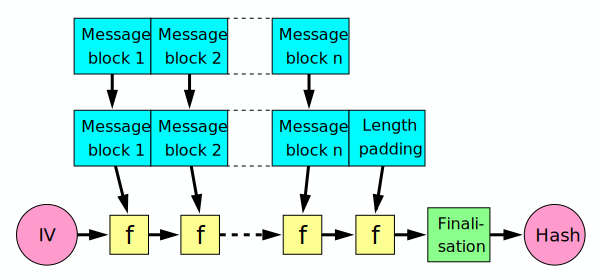
\includegraphics[scale=0.35]{Merkle-Damgard_hash_big}\end{center}
\end{frame}


\begin{frame}
\frametitle{example: SHA-1}
	\begin{itemize}
	\item Blocksize: 512 bit
	\item maximum message length: $2^64-1 bit$
	\end{itemize}
	$f_t(x,y,z) = \left\{ 
	\begin{array}{r@{\quad:\quad}l}
	 -1 & t<0 \\
	  0 & t=0 \\
	  1 & t>0
	\end{array}
	\right. \]$
\end{frame}












